\documentclass[twoside]{book}

% Packages required by doxygen
\usepackage{fixltx2e}
\usepackage{calc}
\usepackage{doxygen}
\usepackage[export]{adjustbox} % also loads graphicx
\usepackage{graphicx}
\usepackage[utf8]{inputenc}
\usepackage{makeidx}
\usepackage{multicol}
\usepackage{multirow}
\PassOptionsToPackage{warn}{textcomp}
\usepackage{textcomp}
\usepackage[nointegrals]{wasysym}
\usepackage[table]{xcolor}

% NLS support packages
\usepackage[spanish]{babel}
% Font selection
\usepackage[T1]{fontenc}
\usepackage[scaled=.90]{helvet}
\usepackage{courier}
\usepackage{amssymb}
\usepackage{sectsty}
\renewcommand{\familydefault}{\sfdefault}
\allsectionsfont{%
  \fontseries{bc}\selectfont%
  \color{darkgray}%
}
\renewcommand{\DoxyLabelFont}{%
  \fontseries{bc}\selectfont%
  \color{darkgray}%
}
\newcommand{\+}{\discretionary{\mbox{\scriptsize$\hookleftarrow$}}{}{}}

% Page & text layout
\usepackage{geometry}
\geometry{%
  a4paper,%
  top=2.5cm,%
  bottom=2.5cm,%
  left=2.5cm,%
  right=2.5cm%
}
\tolerance=750
\hfuzz=15pt
\hbadness=750
\setlength{\emergencystretch}{15pt}
\setlength{\parindent}{0cm}
\setlength{\parskip}{3ex plus 2ex minus 2ex}
\makeatletter
\renewcommand{\paragraph}{%
  \@startsection{paragraph}{4}{0ex}{-1.0ex}{1.0ex}{%
    \normalfont\normalsize\bfseries\SS@parafont%
  }%
}
\renewcommand{\subparagraph}{%
  \@startsection{subparagraph}{5}{0ex}{-1.0ex}{1.0ex}{%
    \normalfont\normalsize\bfseries\SS@subparafont%
  }%
}
\makeatother

% Headers & footers
\usepackage{fancyhdr}
\pagestyle{fancyplain}
\fancyhead[LE]{\fancyplain{}{\bfseries\thepage}}
\fancyhead[CE]{\fancyplain{}{}}
\fancyhead[RE]{\fancyplain{}{\bfseries\leftmark}}
\fancyhead[LO]{\fancyplain{}{\bfseries\rightmark}}
\fancyhead[CO]{\fancyplain{}{}}
\fancyhead[RO]{\fancyplain{}{\bfseries\thepage}}
\fancyfoot[LE]{\fancyplain{}{}}
\fancyfoot[CE]{\fancyplain{}{}}
\fancyfoot[RE]{\fancyplain{}{\bfseries\scriptsize Generado por Doxygen }}
\fancyfoot[LO]{\fancyplain{}{\bfseries\scriptsize Generado por Doxygen }}
\fancyfoot[CO]{\fancyplain{}{}}
\fancyfoot[RO]{\fancyplain{}{}}
\renewcommand{\footrulewidth}{0.4pt}
\renewcommand{\chaptermark}[1]{%
  \markboth{#1}{}%
}
\renewcommand{\sectionmark}[1]{%
  \markright{\thesection\ #1}%
}

% Indices & bibliography
\usepackage{natbib}
\usepackage[titles]{tocloft}
\setcounter{tocdepth}{3}
\setcounter{secnumdepth}{5}
\makeindex

% Hyperlinks (required, but should be loaded last)
\usepackage{ifpdf}
\ifpdf
  \usepackage[pdftex,pagebackref=true]{hyperref}
\else
  \usepackage[ps2pdf,pagebackref=true]{hyperref}
\fi
\hypersetup{%
  colorlinks=true,%
  linkcolor=blue,%
  citecolor=blue,%
  unicode%
}

% Custom commands
\newcommand{\clearemptydoublepage}{%
  \newpage{\pagestyle{empty}\cleardoublepage}%
}

\usepackage{caption}
\captionsetup{labelsep=space,justification=centering,font={bf},singlelinecheck=off,skip=4pt,position=top}

%===== C O N T E N T S =====

\begin{document}

% Titlepage & ToC
\hypersetup{pageanchor=false,
             bookmarksnumbered=true,
             pdfencoding=unicode
            }
\pagenumbering{roman}
\begin{titlepage}
\vspace*{7cm}
\begin{center}%
{\Large Practica 4 }\\
\vspace*{1cm}
{\large Generado por Doxygen 1.8.11}\\
\end{center}
\end{titlepage}
\clearemptydoublepage
\tableofcontents
\clearemptydoublepage
\pagenumbering{arabic}
\hypersetup{pageanchor=true}

%--- Begin generated contents ---
\chapter{Índice de clases}
\section{Lista de clases}
Lista de las clases, estructuras, uniones e interfaces con una breve descripción\+:\begin{DoxyCompactList}
\item\contentsline{section}{\hyperlink{struct__Apuesta}{\+\_\+\+Apuesta} \\*Estructura apuesta }{\pageref{struct__Apuesta}}{}
\item\contentsline{section}{\hyperlink{struct__Caballo}{\+\_\+\+Caballo} \\*Estructura caballo }{\pageref{struct__Caballo}}{}
\item\contentsline{section}{\hyperlink{struct__Carrera}{\+\_\+\+Carrera} \\*Estructura carrera }{\pageref{struct__Carrera}}{}
\item\contentsline{section}{\hyperlink{struct__Mensaje}{\+\_\+\+Mensaje} \\*Estructura mensaje que contiene todos sus parametros necesarios para la realización del ejercicio con colas de mensajes }{\pageref{struct__Mensaje}}{}
\item\contentsline{section}{\hyperlink{struct__Monitor}{\+\_\+\+Monitor} \\*Estructura monitor }{\pageref{struct__Monitor}}{}
\item\contentsline{section}{\hyperlink{struct__Ventanilla}{\+\_\+\+Ventanilla} \\*Estructura ventanilla }{\pageref{struct__Ventanilla}}{}
\end{DoxyCompactList}

\chapter{Indice de archivos}
\section{Lista de archivos}
Lista de todos los archivos documentados y con descripciones breves\+:\begin{DoxyCompactList}
\item\contentsline{section}{\hyperlink{ejercicio10_8c}{ejercicio10.\+c} \\*Implementa el ejercicio 10 de mascaras }{\pageref{ejercicio10_8c}}{}
\item\contentsline{section}{\hyperlink{ejercicio3a_8c}{ejercicio3a.\+c} \\*Implementa el ejercicio 3a de procesos con un solo padre }{\pageref{ejercicio3a_8c}}{}
\item\contentsline{section}{\hyperlink{ejercicio3b_8c}{ejercicio3b.\+c} \\*Implementa el ejercicio 3b de hilos de un proceso }{\pageref{ejercicio3b_8c}}{}
\item\contentsline{section}{\hyperlink{ejercicio4a_8c}{ejercicio4a.\+c} \\*Implementa el ejercicio 4a de multiplicacion de matrices }{\pageref{ejercicio4a_8c}}{}
\item\contentsline{section}{\hyperlink{ejercicio4b_8c}{ejercicio4b.\+c} \\*Implementa el ejercicio 4b de multiplicacion de matrices }{\pageref{ejercicio4b_8c}}{}
\item\contentsline{section}{\hyperlink{ejercicio6_8c}{ejercicio6.\+c} \\*Implementa el ejercicio 6 de señales }{\pageref{ejercicio6_8c}}{}
\end{DoxyCompactList}

\chapter{Documentación de las clases}
\hypertarget{struct__Apuesta}{}\section{Referencia de la Estructura \+\_\+\+Apuesta}
\label{struct__Apuesta}\index{\+\_\+\+Apuesta@{\+\_\+\+Apuesta}}


Estructura apuesta.  


\subsection*{Atributos públicos}
\begin{DoxyCompactItemize}
\item 
long \hyperlink{struct__Apuesta_aaa377830ba615faf9c7cb0bdbb8554e5}{id}
\item 
char \hyperlink{struct__Apuesta_ae4d7fe3277098d3c32d34b435408873e}{nombre} \mbox{[}20\mbox{]}
\item 
int \hyperlink{struct__Apuesta_a217a68a637b2db3e61068bafc18ef1ac}{num\+Caballo}
\item 
double \hyperlink{struct__Apuesta_a905f551e1d83b725da8f1e10ab787193}{cuantia}
\end{DoxyCompactItemize}


\subsection{Descripción detallada}
Estructura apuesta. 

\subsection{Documentación de los datos miembro}
\index{\+\_\+\+Apuesta@{\+\_\+\+Apuesta}!cuantia@{cuantia}}
\index{cuantia@{cuantia}!\+\_\+\+Apuesta@{\+\_\+\+Apuesta}}
\subsubsection[{\texorpdfstring{cuantia}{cuantia}}]{\setlength{\rightskip}{0pt plus 5cm}double \+\_\+\+Apuesta\+::cuantia}\hypertarget{struct__Apuesta_a905f551e1d83b725da8f1e10ab787193}{}\label{struct__Apuesta_a905f551e1d83b725da8f1e10ab787193}
Total apostado \index{\+\_\+\+Apuesta@{\+\_\+\+Apuesta}!id@{id}}
\index{id@{id}!\+\_\+\+Apuesta@{\+\_\+\+Apuesta}}
\subsubsection[{\texorpdfstring{id}{id}}]{\setlength{\rightskip}{0pt plus 5cm}long \+\_\+\+Apuesta\+::id}\hypertarget{struct__Apuesta_aaa377830ba615faf9c7cb0bdbb8554e5}{}\label{struct__Apuesta_aaa377830ba615faf9c7cb0bdbb8554e5}
Tipo de mensaje \index{\+\_\+\+Apuesta@{\+\_\+\+Apuesta}!nombre@{nombre}}
\index{nombre@{nombre}!\+\_\+\+Apuesta@{\+\_\+\+Apuesta}}
\subsubsection[{\texorpdfstring{nombre}{nombre}}]{\setlength{\rightskip}{0pt plus 5cm}char \+\_\+\+Apuesta\+::nombre\mbox{[}20\mbox{]}}\hypertarget{struct__Apuesta_ae4d7fe3277098d3c32d34b435408873e}{}\label{struct__Apuesta_ae4d7fe3277098d3c32d34b435408873e}
Nombre del apostador \index{\+\_\+\+Apuesta@{\+\_\+\+Apuesta}!num\+Caballo@{num\+Caballo}}
\index{num\+Caballo@{num\+Caballo}!\+\_\+\+Apuesta@{\+\_\+\+Apuesta}}
\subsubsection[{\texorpdfstring{num\+Caballo}{numCaballo}}]{\setlength{\rightskip}{0pt plus 5cm}int \+\_\+\+Apuesta\+::num\+Caballo}\hypertarget{struct__Apuesta_a217a68a637b2db3e61068bafc18ef1ac}{}\label{struct__Apuesta_a217a68a637b2db3e61068bafc18ef1ac}
Numero del caballo que apuesta 

La documentación para esta estructura fue generada a partir del siguiente fichero\+:\begin{DoxyCompactItemize}
\item 
\hyperlink{carrera_8c}{carrera.\+c}\end{DoxyCompactItemize}

\hypertarget{struct__Caballo}{}\section{Referencia de la Estructura \+\_\+\+Caballo}
\label{struct__Caballo}\index{\+\_\+\+Caballo@{\+\_\+\+Caballo}}


Estructura caballo.  


\subsection*{Atributos públicos}
\begin{DoxyCompactItemize}
\item 
int \hyperlink{struct__Caballo_a233e3c2f3372a27dcff1e4161cbb9ff4}{id}
\item 
double \hyperlink{struct__Caballo_ac18791b370ba0dfbf8bb29554e701cb3}{totalapostado}
\item 
double \hyperlink{struct__Caballo_a69f38b3e2d3718a80b71b5384ab7ffb8}{cotizacion}
\end{DoxyCompactItemize}


\subsection{Descripción detallada}
Estructura caballo. 

\subsection{Documentación de los datos miembro}
\index{\+\_\+\+Caballo@{\+\_\+\+Caballo}!cotizacion@{cotizacion}}
\index{cotizacion@{cotizacion}!\+\_\+\+Caballo@{\+\_\+\+Caballo}}
\subsubsection[{\texorpdfstring{cotizacion}{cotizacion}}]{\setlength{\rightskip}{0pt plus 5cm}double \+\_\+\+Caballo\+::cotizacion}\hypertarget{struct__Caballo_a69f38b3e2d3718a80b71b5384ab7ffb8}{}\label{struct__Caballo_a69f38b3e2d3718a80b71b5384ab7ffb8}
Cotizacion del caballo \index{\+\_\+\+Caballo@{\+\_\+\+Caballo}!id@{id}}
\index{id@{id}!\+\_\+\+Caballo@{\+\_\+\+Caballo}}
\subsubsection[{\texorpdfstring{id}{id}}]{\setlength{\rightskip}{0pt plus 5cm}int \+\_\+\+Caballo\+::id}\hypertarget{struct__Caballo_a233e3c2f3372a27dcff1e4161cbb9ff4}{}\label{struct__Caballo_a233e3c2f3372a27dcff1e4161cbb9ff4}
Identificador del caballo \index{\+\_\+\+Caballo@{\+\_\+\+Caballo}!totalapostado@{totalapostado}}
\index{totalapostado@{totalapostado}!\+\_\+\+Caballo@{\+\_\+\+Caballo}}
\subsubsection[{\texorpdfstring{totalapostado}{totalapostado}}]{\setlength{\rightskip}{0pt plus 5cm}double \+\_\+\+Caballo\+::totalapostado}\hypertarget{struct__Caballo_ac18791b370ba0dfbf8bb29554e701cb3}{}\label{struct__Caballo_ac18791b370ba0dfbf8bb29554e701cb3}
Total Dinero apostado al caballo 

La documentación para esta estructura fue generada a partir del siguiente fichero\+:\begin{DoxyCompactItemize}
\item 
\hyperlink{carrera_8c}{carrera.\+c}\end{DoxyCompactItemize}

\hypertarget{struct__Carrera}{}\section{Referencia de la Estructura \+\_\+\+Carrera}
\label{struct__Carrera}\index{\+\_\+\+Carrera@{\+\_\+\+Carrera}}


Estructura carrera.  


\subsection*{Atributos públicos}
\begin{DoxyCompactItemize}
\item 
int \hyperlink{struct__Carrera_a842fb73a7e5fd05a5c80079b67eac95b}{id}
\item 
int \hyperlink{struct__Carrera_aae30a3f276a9ac25ffa42fa65736a735}{pid}
\item 
int \hyperlink{struct__Carrera_a2c723a949d2125c8989fabf48028ba12}{pos}
\item 
int \hyperlink{struct__Carrera_ae091854540d0a874642d92c971a0f86a}{tirada}
\end{DoxyCompactItemize}


\subsection{Descripción detallada}
Estructura carrera. 

\subsection{Documentación de los datos miembro}
\index{\+\_\+\+Carrera@{\+\_\+\+Carrera}!id@{id}}
\index{id@{id}!\+\_\+\+Carrera@{\+\_\+\+Carrera}}
\subsubsection[{\texorpdfstring{id}{id}}]{\setlength{\rightskip}{0pt plus 5cm}int \+\_\+\+Carrera\+::id}\hypertarget{struct__Carrera_a842fb73a7e5fd05a5c80079b67eac95b}{}\label{struct__Carrera_a842fb73a7e5fd05a5c80079b67eac95b}
id del caballo de 1 hasta el numero de caballos \index{\+\_\+\+Carrera@{\+\_\+\+Carrera}!pid@{pid}}
\index{pid@{pid}!\+\_\+\+Carrera@{\+\_\+\+Carrera}}
\subsubsection[{\texorpdfstring{pid}{pid}}]{\setlength{\rightskip}{0pt plus 5cm}int \+\_\+\+Carrera\+::pid}\hypertarget{struct__Carrera_aae30a3f276a9ac25ffa42fa65736a735}{}\label{struct__Carrera_aae30a3f276a9ac25ffa42fa65736a735}
pid del proceso correspondiente a este caballo \index{\+\_\+\+Carrera@{\+\_\+\+Carrera}!pos@{pos}}
\index{pos@{pos}!\+\_\+\+Carrera@{\+\_\+\+Carrera}}
\subsubsection[{\texorpdfstring{pos}{pos}}]{\setlength{\rightskip}{0pt plus 5cm}int \+\_\+\+Carrera\+::pos}\hypertarget{struct__Carrera_a2c723a949d2125c8989fabf48028ba12}{}\label{struct__Carrera_a2c723a949d2125c8989fabf48028ba12}
posicion de este caballo \index{\+\_\+\+Carrera@{\+\_\+\+Carrera}!tirada@{tirada}}
\index{tirada@{tirada}!\+\_\+\+Carrera@{\+\_\+\+Carrera}}
\subsubsection[{\texorpdfstring{tirada}{tirada}}]{\setlength{\rightskip}{0pt plus 5cm}int \+\_\+\+Carrera\+::tirada}\hypertarget{struct__Carrera_ae091854540d0a874642d92c971a0f86a}{}\label{struct__Carrera_ae091854540d0a874642d92c971a0f86a}
tiradas de este caballo 

La documentación para esta estructura fue generada a partir del siguiente fichero\+:\begin{DoxyCompactItemize}
\item 
\hyperlink{carrera_8c}{carrera.\+c}\end{DoxyCompactItemize}

\hypertarget{struct__Mensaje}{}\section{Referencia de la Estructura \+\_\+\+Mensaje}
\label{struct__Mensaje}\index{\+\_\+\+Mensaje@{\+\_\+\+Mensaje}}


Estructura mensaje que contiene todos sus parametros necesarios para la realización del ejercicio con colas de mensajes.  


\subsection*{Atributos públicos}
\begin{DoxyCompactItemize}
\item 
long \hyperlink{struct__Mensaje_a216a370cde3eae04df6a81fea5bef338}{id}
\item 
char \hyperlink{struct__Mensaje_a4187bae10cdeba06a6a99d6d57e85a54}{aviso} \mbox{[}\hyperlink{cadena__montaje_8c_a0e68c4ad6b4b3a349afa80ebbbdffb13}{M\+A\+X\+T\+AM}\mbox{]}
\end{DoxyCompactItemize}


\subsection{Descripción detallada}
Estructura mensaje que contiene todos sus parametros necesarios para la realización del ejercicio con colas de mensajes. 

\subsection{Documentación de los datos miembro}
\index{\+\_\+\+Mensaje@{\+\_\+\+Mensaje}!aviso@{aviso}}
\index{aviso@{aviso}!\+\_\+\+Mensaje@{\+\_\+\+Mensaje}}
\subsubsection[{\texorpdfstring{aviso}{aviso}}]{\setlength{\rightskip}{0pt plus 5cm}char \+\_\+\+Mensaje\+::aviso\mbox{[}{\bf M\+A\+X\+T\+AM}\mbox{]}}\hypertarget{struct__Mensaje_a4187bae10cdeba06a6a99d6d57e85a54}{}\label{struct__Mensaje_a4187bae10cdeba06a6a99d6d57e85a54}
Tamanyo maximo aviso \index{\+\_\+\+Mensaje@{\+\_\+\+Mensaje}!id@{id}}
\index{id@{id}!\+\_\+\+Mensaje@{\+\_\+\+Mensaje}}
\subsubsection[{\texorpdfstring{id}{id}}]{\setlength{\rightskip}{0pt plus 5cm}long \+\_\+\+Mensaje\+::id}\hypertarget{struct__Mensaje_a216a370cde3eae04df6a81fea5bef338}{}\label{struct__Mensaje_a216a370cde3eae04df6a81fea5bef338}
Tipo de mensaje 

La documentación para esta estructura fue generada a partir del siguiente fichero\+:\begin{DoxyCompactItemize}
\item 
\hyperlink{cadena__montaje_8c}{cadena\+\_\+montaje.\+c}\end{DoxyCompactItemize}

\hypertarget{struct__Monitor}{}\section{Referencia de la Estructura \+\_\+\+Monitor}
\label{struct__Monitor}\index{\+\_\+\+Monitor@{\+\_\+\+Monitor}}


Estructura monitor.  




Diagrama de colaboración para \+\_\+\+Monitor\+:\nopagebreak
\begin{figure}[H]
\begin{center}
\leavevmode
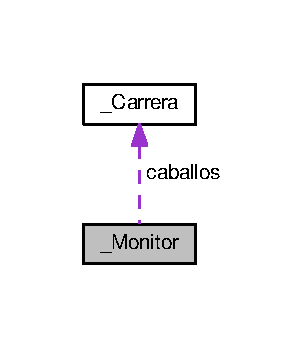
\includegraphics[width=147pt]{struct__Monitor__coll__graph}
\end{center}
\end{figure}
\subsection*{Atributos públicos}
\begin{DoxyCompactItemize}
\item 
int $\ast$ \hyperlink{struct__Monitor_a8c99fc7fcd474a35e14047b2d46af390}{j}
\item 
int $\ast$ \hyperlink{struct__Monitor_ae06ed31d1e98a347e8147b713551fa26}{k}
\item 
int \hyperlink{struct__Monitor_aa927c580f30b2085647032599b6dde4c}{shmid}
\item 
int \hyperlink{struct__Monitor_a5a1c304eaa4f2cca52dc2d5ac937894e}{num\+Caballos}
\item 
int \hyperlink{struct__Monitor_a54944b0b93b7d647fed1a5225e02d40a}{num\+Apostadores}
\item 
\hyperlink{carrera_8c_a33c95e52916a47e1884db1151b066166}{carrera} $\ast$ \hyperlink{struct__Monitor_a4c856b284d47e65fddfa0b3898895489}{caballos}
\end{DoxyCompactItemize}


\subsection{Descripción detallada}
Estructura monitor. 

\subsection{Documentación de los datos miembro}
\index{\+\_\+\+Monitor@{\+\_\+\+Monitor}!caballos@{caballos}}
\index{caballos@{caballos}!\+\_\+\+Monitor@{\+\_\+\+Monitor}}
\subsubsection[{\texorpdfstring{caballos}{caballos}}]{\setlength{\rightskip}{0pt plus 5cm}{\bf carrera}$\ast$ \+\_\+\+Monitor\+::caballos}\hypertarget{struct__Monitor_a4c856b284d47e65fddfa0b3898895489}{}\label{struct__Monitor_a4c856b284d47e65fddfa0b3898895489}
array de la estructura carrera para cada caballo \index{\+\_\+\+Monitor@{\+\_\+\+Monitor}!j@{j}}
\index{j@{j}!\+\_\+\+Monitor@{\+\_\+\+Monitor}}
\subsubsection[{\texorpdfstring{j}{j}}]{\setlength{\rightskip}{0pt plus 5cm}int$\ast$ \+\_\+\+Monitor\+::j}\hypertarget{struct__Monitor_a8c99fc7fcd474a35e14047b2d46af390}{}\label{struct__Monitor_a8c99fc7fcd474a35e14047b2d46af390}
Sincronizacion entre proceso padre e hijo \index{\+\_\+\+Monitor@{\+\_\+\+Monitor}!k@{k}}
\index{k@{k}!\+\_\+\+Monitor@{\+\_\+\+Monitor}}
\subsubsection[{\texorpdfstring{k}{k}}]{\setlength{\rightskip}{0pt plus 5cm}int$\ast$ \+\_\+\+Monitor\+::k}\hypertarget{struct__Monitor_ae06ed31d1e98a347e8147b713551fa26}{}\label{struct__Monitor_ae06ed31d1e98a347e8147b713551fa26}
Sincronizacion entre proceso padre e hijo \index{\+\_\+\+Monitor@{\+\_\+\+Monitor}!num\+Apostadores@{num\+Apostadores}}
\index{num\+Apostadores@{num\+Apostadores}!\+\_\+\+Monitor@{\+\_\+\+Monitor}}
\subsubsection[{\texorpdfstring{num\+Apostadores}{numApostadores}}]{\setlength{\rightskip}{0pt plus 5cm}int \+\_\+\+Monitor\+::num\+Apostadores}\hypertarget{struct__Monitor_a54944b0b93b7d647fed1a5225e02d40a}{}\label{struct__Monitor_a54944b0b93b7d647fed1a5225e02d40a}
numero de apostadores \index{\+\_\+\+Monitor@{\+\_\+\+Monitor}!num\+Caballos@{num\+Caballos}}
\index{num\+Caballos@{num\+Caballos}!\+\_\+\+Monitor@{\+\_\+\+Monitor}}
\subsubsection[{\texorpdfstring{num\+Caballos}{numCaballos}}]{\setlength{\rightskip}{0pt plus 5cm}int \+\_\+\+Monitor\+::num\+Caballos}\hypertarget{struct__Monitor_a5a1c304eaa4f2cca52dc2d5ac937894e}{}\label{struct__Monitor_a5a1c304eaa4f2cca52dc2d5ac937894e}
numero de caballos \index{\+\_\+\+Monitor@{\+\_\+\+Monitor}!shmid@{shmid}}
\index{shmid@{shmid}!\+\_\+\+Monitor@{\+\_\+\+Monitor}}
\subsubsection[{\texorpdfstring{shmid}{shmid}}]{\setlength{\rightskip}{0pt plus 5cm}int \+\_\+\+Monitor\+::shmid}\hypertarget{struct__Monitor_aa927c580f30b2085647032599b6dde4c}{}\label{struct__Monitor_aa927c580f30b2085647032599b6dde4c}
Identificador de la memoria compartida 

La documentación para esta estructura fue generada a partir del siguiente fichero\+:\begin{DoxyCompactItemize}
\item 
\hyperlink{carrera_8c}{carrera.\+c}\end{DoxyCompactItemize}

\hypertarget{struct__Ventanilla}{}\section{Referencia de la Estructura \+\_\+\+Ventanilla}
\label{struct__Ventanilla}\index{\+\_\+\+Ventanilla@{\+\_\+\+Ventanilla}}


Estructura ventanilla.  




Diagrama de colaboración para \+\_\+\+Ventanilla\+:\nopagebreak
\begin{figure}[H]
\begin{center}
\leavevmode
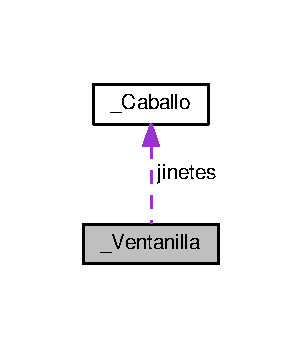
\includegraphics[width=145pt]{struct__Ventanilla__coll__graph}
\end{center}
\end{figure}
\subsection*{Atributos públicos}
\begin{DoxyCompactItemize}
\item 
int \hyperlink{struct__Ventanilla_a9d1361c0811ea37ac86765ed0ad50a8f}{num\+Caballos}
\item 
\hyperlink{carrera_8c_a9700d9b08f47d213e0daf7317219022e}{caballo} \hyperlink{struct__Ventanilla_ab359f2cc43a4adf0b65ccf8ffd5cd145}{jinetes} \mbox{[}\hyperlink{carrera_8c_a392fb874e547e582e9c66a08a1f23326}{M\+AX}\mbox{]}
\item 
double \hyperlink{struct__Ventanilla_a19ef890de873fe54c27d1726fb9ca947}{apostadores} \mbox{[}\hyperlink{carrera_8c_a392fb874e547e582e9c66a08a1f23326}{M\+AX}\mbox{]}\mbox{[}\hyperlink{carrera_8c_a392fb874e547e582e9c66a08a1f23326}{M\+AX}\mbox{]}
\item 
double \hyperlink{struct__Ventanilla_a1b4846eb8da9d38419a3f918fe9665c1}{total}
\item 
int \hyperlink{struct__Ventanilla_a66a8337f17a857c1ad379db598bba1c9}{msgid}
\item 
int \hyperlink{struct__Ventanilla_a2834f69015926e1879286fe9af2a72b3}{semid}
\item 
int \hyperlink{struct__Ventanilla_a6b5316b20a1be71403695aeac94346e5}{estado}
\end{DoxyCompactItemize}


\subsection{Descripción detallada}
Estructura ventanilla. 

\subsection{Documentación de los datos miembro}
\index{\+\_\+\+Ventanilla@{\+\_\+\+Ventanilla}!apostadores@{apostadores}}
\index{apostadores@{apostadores}!\+\_\+\+Ventanilla@{\+\_\+\+Ventanilla}}
\subsubsection[{\texorpdfstring{apostadores}{apostadores}}]{\setlength{\rightskip}{0pt plus 5cm}double \+\_\+\+Ventanilla\+::apostadores\mbox{[}{\bf M\+AX}\mbox{]}\mbox{[}{\bf M\+AX}\mbox{]}}\hypertarget{struct__Ventanilla_a19ef890de873fe54c27d1726fb9ca947}{}\label{struct__Ventanilla_a19ef890de873fe54c27d1726fb9ca947}
matriz de apostadores-\/caballo \index{\+\_\+\+Ventanilla@{\+\_\+\+Ventanilla}!estado@{estado}}
\index{estado@{estado}!\+\_\+\+Ventanilla@{\+\_\+\+Ventanilla}}
\subsubsection[{\texorpdfstring{estado}{estado}}]{\setlength{\rightskip}{0pt plus 5cm}int \+\_\+\+Ventanilla\+::estado}\hypertarget{struct__Ventanilla_a6b5316b20a1be71403695aeac94346e5}{}\label{struct__Ventanilla_a6b5316b20a1be71403695aeac94346e5}
estado de la carrera \index{\+\_\+\+Ventanilla@{\+\_\+\+Ventanilla}!jinetes@{jinetes}}
\index{jinetes@{jinetes}!\+\_\+\+Ventanilla@{\+\_\+\+Ventanilla}}
\subsubsection[{\texorpdfstring{jinetes}{jinetes}}]{\setlength{\rightskip}{0pt plus 5cm}{\bf caballo} \+\_\+\+Ventanilla\+::jinetes\mbox{[}{\bf M\+AX}\mbox{]}}\hypertarget{struct__Ventanilla_ab359f2cc43a4adf0b65ccf8ffd5cd145}{}\label{struct__Ventanilla_ab359f2cc43a4adf0b65ccf8ffd5cd145}
array de punteros a la estructura de caballo \index{\+\_\+\+Ventanilla@{\+\_\+\+Ventanilla}!msgid@{msgid}}
\index{msgid@{msgid}!\+\_\+\+Ventanilla@{\+\_\+\+Ventanilla}}
\subsubsection[{\texorpdfstring{msgid}{msgid}}]{\setlength{\rightskip}{0pt plus 5cm}int \+\_\+\+Ventanilla\+::msgid}\hypertarget{struct__Ventanilla_a66a8337f17a857c1ad379db598bba1c9}{}\label{struct__Ventanilla_a66a8337f17a857c1ad379db598bba1c9}
id de la cola de mensajes \index{\+\_\+\+Ventanilla@{\+\_\+\+Ventanilla}!num\+Caballos@{num\+Caballos}}
\index{num\+Caballos@{num\+Caballos}!\+\_\+\+Ventanilla@{\+\_\+\+Ventanilla}}
\subsubsection[{\texorpdfstring{num\+Caballos}{numCaballos}}]{\setlength{\rightskip}{0pt plus 5cm}int \+\_\+\+Ventanilla\+::num\+Caballos}\hypertarget{struct__Ventanilla_a9d1361c0811ea37ac86765ed0ad50a8f}{}\label{struct__Ventanilla_a9d1361c0811ea37ac86765ed0ad50a8f}
numero de caballos \index{\+\_\+\+Ventanilla@{\+\_\+\+Ventanilla}!semid@{semid}}
\index{semid@{semid}!\+\_\+\+Ventanilla@{\+\_\+\+Ventanilla}}
\subsubsection[{\texorpdfstring{semid}{semid}}]{\setlength{\rightskip}{0pt plus 5cm}int \+\_\+\+Ventanilla\+::semid}\hypertarget{struct__Ventanilla_a2834f69015926e1879286fe9af2a72b3}{}\label{struct__Ventanilla_a2834f69015926e1879286fe9af2a72b3}
id del array de semaforos \index{\+\_\+\+Ventanilla@{\+\_\+\+Ventanilla}!total@{total}}
\index{total@{total}!\+\_\+\+Ventanilla@{\+\_\+\+Ventanilla}}
\subsubsection[{\texorpdfstring{total}{total}}]{\setlength{\rightskip}{0pt plus 5cm}double \+\_\+\+Ventanilla\+::total}\hypertarget{struct__Ventanilla_a1b4846eb8da9d38419a3f918fe9665c1}{}\label{struct__Ventanilla_a1b4846eb8da9d38419a3f918fe9665c1}
total apostado a todos los caballos 

La documentación para esta estructura fue generada a partir del siguiente fichero\+:\begin{DoxyCompactItemize}
\item 
\hyperlink{carrera_8c}{carrera.\+c}\end{DoxyCompactItemize}

\chapter{Documentación de archivos}
\hypertarget{cadena__montaje_8c}{}\section{Referencia del Archivo cadena\+\_\+montaje.\+c}
\label{cadena__montaje_8c}\index{cadena\+\_\+montaje.\+c@{cadena\+\_\+montaje.\+c}}


Implementa el ejercicio \hyperlink{cadena__montaje_8c}{cadena\+\_\+montaje.\+c} de mensajes.  


{\ttfamily \#include $<$stdio.\+h$>$}\\*
{\ttfamily \#include $<$stdlib.\+h$>$}\\*
{\ttfamily \#include $<$string.\+h$>$}\\*
{\ttfamily \#include $<$sys/types.\+h$>$}\\*
{\ttfamily \#include $<$sys/ipc.\+h$>$}\\*
{\ttfamily \#include $<$sys/msg.\+h$>$}\\*
{\ttfamily \#include $<$signal.\+h$>$}\\*
{\ttfamily \#include $<$sys/shm.\+h$>$}\\*
{\ttfamily \#include $<$sys/wait.\+h$>$}\\*
{\ttfamily \#include $<$errno.\+h$>$}\\*
{\ttfamily \#include $<$unistd.\+h$>$}\\*
{\ttfamily \#include $<$math.\+h$>$}\\*
Dependencia gráfica adjunta para cadena\+\_\+montaje.\+c\+:\nopagebreak
\begin{figure}[H]
\begin{center}
\leavevmode
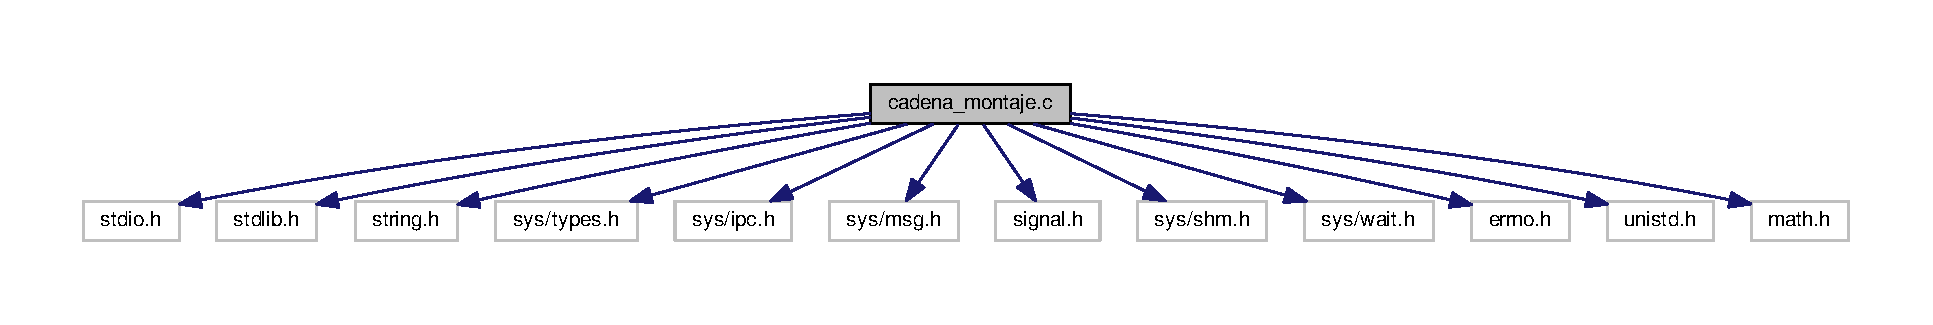
\includegraphics[width=350pt]{cadena__montaje_8c__incl}
\end{center}
\end{figure}
\subsection*{Clases}
\begin{DoxyCompactItemize}
\item 
struct \hyperlink{struct__Mensaje}{\+\_\+\+Mensaje}
\begin{DoxyCompactList}\small\item\em Estructura mensaje que contiene todos sus parametros necesarios para la realización del ejercicio con colas de mensajes. \end{DoxyCompactList}\end{DoxyCompactItemize}
\subsection*{\textquotesingle{}defines\textquotesingle{}}
\begin{DoxyCompactItemize}
\item 
\#define \hyperlink{cadena__montaje_8c_a8ae9d53f33f46cfcfcb9736e6351452a}{K\+EY}~1300\hypertarget{cadena__montaje_8c_a8ae9d53f33f46cfcfcb9736e6351452a}{}\label{cadena__montaje_8c_a8ae9d53f33f46cfcfcb9736e6351452a}

\begin{DoxyCompactList}\small\item\em Definicion de la clave. \end{DoxyCompactList}\item 
\#define \hyperlink{cadena__montaje_8c_a68c15c5fb7f7c6f707903e6a46ab0557}{F\+I\+L\+E\+K\+EY}~\char`\"{}/bin/cat\char`\"{}\hypertarget{cadena__montaje_8c_a68c15c5fb7f7c6f707903e6a46ab0557}{}\label{cadena__montaje_8c_a68c15c5fb7f7c6f707903e6a46ab0557}

\begin{DoxyCompactList}\small\item\em Definicion de la clave de fichero. \end{DoxyCompactList}\item 
\#define \hyperlink{cadena__montaje_8c_a1a96b801681f9111bd2f315be7254984}{N\+U\+M\+\_\+\+P\+R\+O\+C\+E\+S\+OS}~3\hypertarget{cadena__montaje_8c_a1a96b801681f9111bd2f315be7254984}{}\label{cadena__montaje_8c_a1a96b801681f9111bd2f315be7254984}

\begin{DoxyCompactList}\small\item\em Definicion del numero de procesos hijos totales. \end{DoxyCompactList}\item 
\#define \hyperlink{cadena__montaje_8c_a0e68c4ad6b4b3a349afa80ebbbdffb13}{M\+A\+X\+T\+AM}~4096\hypertarget{cadena__montaje_8c_a0e68c4ad6b4b3a349afa80ebbbdffb13}{}\label{cadena__montaje_8c_a0e68c4ad6b4b3a349afa80ebbbdffb13}

\begin{DoxyCompactList}\small\item\em Definicion del tamanyo maximo de lectura del fichero. \end{DoxyCompactList}\end{DoxyCompactItemize}
\subsection*{\textquotesingle{}typedefs\textquotesingle{}}
\begin{DoxyCompactItemize}
\item 
typedef struct \hyperlink{struct__Mensaje}{\+\_\+\+Mensaje} \hyperlink{cadena__montaje_8c_a59d8c217fe65b74ca325b7796b8d5e7c}{mensaje}\hypertarget{cadena__montaje_8c_a59d8c217fe65b74ca325b7796b8d5e7c}{}\label{cadena__montaje_8c_a59d8c217fe65b74ca325b7796b8d5e7c}

\begin{DoxyCompactList}\small\item\em Estructura mensaje que contiene todos sus parametros necesarios para la realización del ejercicio con colas de mensajes. \end{DoxyCompactList}\end{DoxyCompactItemize}
\subsection*{Funciones}
\begin{DoxyCompactItemize}
\item 
int \hyperlink{cadena__montaje_8c_a0ddf1224851353fc92bfbff6f499fa97}{main} (int argc, char $\ast$argv\mbox{[}$\,$\mbox{]})
\begin{DoxyCompactList}\small\item\em funcion principal que pide un fichero de entrada y otro de salida y realiza el paso de mensajes pedidos \end{DoxyCompactList}\end{DoxyCompactItemize}


\subsection{Descripción detallada}
Implementa el ejercicio \hyperlink{cadena__montaje_8c}{cadena\+\_\+montaje.\+c} de mensajes. 

\begin{DoxyAuthor}{Autor}
Andres Salas \href{mailto:andres.salas@estudiante.uam.es}{\tt andres.\+salas@estudiante.\+uam.\+es} 

Antonio Martin \href{mailto:antonio.martinmasuda@estudiante.uam.es}{\tt antonio.\+martinmasuda@estudiante.\+uam.\+es} 
\end{DoxyAuthor}
\begin{DoxyNote}{Nota}
Grupo 2202 
\end{DoxyNote}
\begin{DoxyVersion}{Versión}
1.\+0 
\end{DoxyVersion}
\begin{DoxyDate}{Fecha}
8/04/2017 
\end{DoxyDate}


\subsection{Documentación de las funciones}
\index{cadena\+\_\+montaje.\+c@{cadena\+\_\+montaje.\+c}!main@{main}}
\index{main@{main}!cadena\+\_\+montaje.\+c@{cadena\+\_\+montaje.\+c}}
\subsubsection[{\texorpdfstring{main(int argc, char $\ast$argv[])}{main(int argc, char *argv[])}}]{\setlength{\rightskip}{0pt plus 5cm}int main (
\begin{DoxyParamCaption}
\item[{int}]{argc, }
\item[{char $\ast$}]{argv\mbox{[}$\,$\mbox{]}}
\end{DoxyParamCaption}
)}\hypertarget{cadena__montaje_8c_a0ddf1224851353fc92bfbff6f499fa97}{}\label{cadena__montaje_8c_a0ddf1224851353fc92bfbff6f499fa97}


funcion principal que pide un fichero de entrada y otro de salida y realiza el paso de mensajes pedidos 


\begin{DoxyParams}{Parámetros}
{\em argc} & contiene el número de parámetros totales pasados \\
\hline
{\em argv} & contiene los parámetros pasados por el usuario \\
\hline
\end{DoxyParams}
\begin{DoxyReturn}{Devuelve}
int\+: valor de exito (OK) o fracaso (E\+R\+R\+OR) 
\end{DoxyReturn}

\hypertarget{carrera_8c}{}\section{Referencia del Archivo carrera.\+c}
\label{carrera_8c}\index{carrera.\+c@{carrera.\+c}}


Implementa el ejercicio \hyperlink{carrera_8c}{carrera.\+c} que engloba todos los contenidos.  


{\ttfamily \#include $<$stdio.\+h$>$}\\*
{\ttfamily \#include $<$stdlib.\+h$>$}\\*
{\ttfamily \#include $<$string.\+h$>$}\\*
{\ttfamily \#include $<$sys/wait.\+h$>$}\\*
{\ttfamily \#include $<$signal.\+h$>$}\\*
{\ttfamily \#include $<$sys/shm.\+h$>$}\\*
{\ttfamily \#include $<$sys/sem.\+h$>$}\\*
{\ttfamily \#include $<$sys/types.\+h$>$}\\*
{\ttfamily \#include $<$sys/ipc.\+h$>$}\\*
{\ttfamily \#include $<$unistd.\+h$>$}\\*
{\ttfamily \#include $<$pthread.\+h$>$}\\*
{\ttfamily \#include $<$sys/msg.\+h$>$}\\*
{\ttfamily \#include $<$errno.\+h$>$}\\*
{\ttfamily \#include $<$time.\+h$>$}\\*
Dependencia gráfica adjunta para carrera.\+c\+:\nopagebreak
\begin{figure}[H]
\begin{center}
\leavevmode
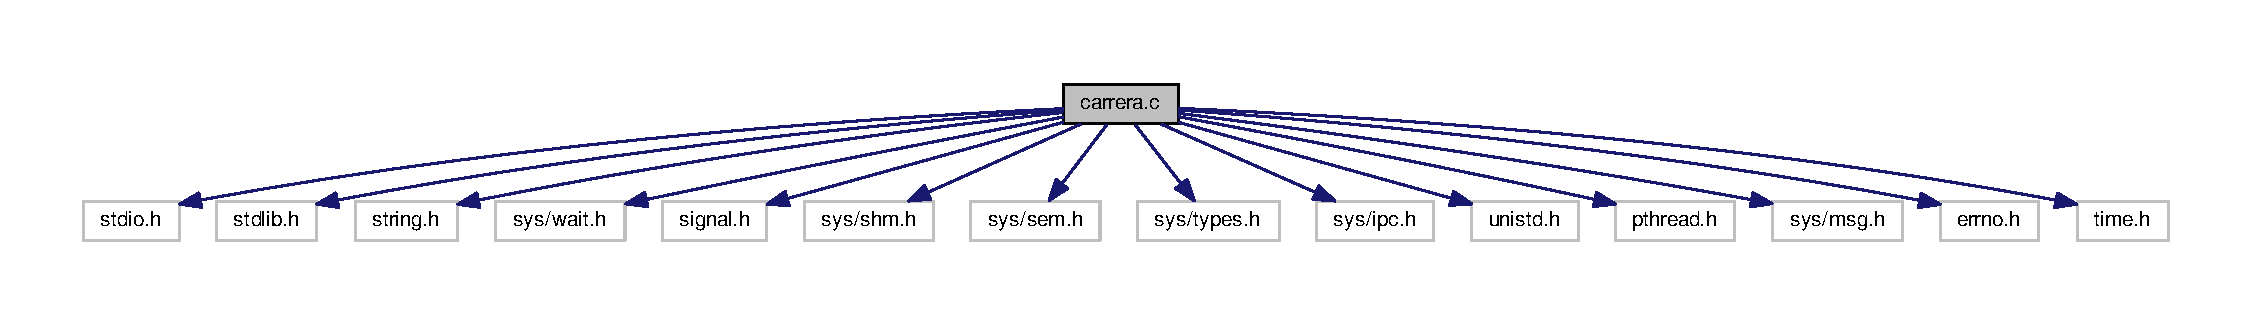
\includegraphics[width=350pt]{carrera_8c__incl}
\end{center}
\end{figure}
\subsection*{Clases}
\begin{DoxyCompactItemize}
\item 
struct \hyperlink{struct__Apuesta}{\+\_\+\+Apuesta}
\begin{DoxyCompactList}\small\item\em Estructura apuesta. \end{DoxyCompactList}\item 
struct \hyperlink{struct__Caballo}{\+\_\+\+Caballo}
\begin{DoxyCompactList}\small\item\em Estructura caballo. \end{DoxyCompactList}\item 
struct \hyperlink{struct__Carrera}{\+\_\+\+Carrera}
\begin{DoxyCompactList}\small\item\em Estructura carrera. \end{DoxyCompactList}\item 
struct \hyperlink{struct__Ventanilla}{\+\_\+\+Ventanilla}
\begin{DoxyCompactList}\small\item\em Estructura ventanilla. \end{DoxyCompactList}\item 
struct \hyperlink{struct__Monitor}{\+\_\+\+Monitor}
\begin{DoxyCompactList}\small\item\em Estructura monitor. \end{DoxyCompactList}\end{DoxyCompactItemize}
\subsection*{\textquotesingle{}defines\textquotesingle{}}
\begin{DoxyCompactItemize}
\item 
\#define \hyperlink{carrera_8c_abc8a865f8ec2f1343ebeded8e37b47dc}{L\+E\+ER}~0\hypertarget{carrera_8c_abc8a865f8ec2f1343ebeded8e37b47dc}{}\label{carrera_8c_abc8a865f8ec2f1343ebeded8e37b47dc}

\begin{DoxyCompactList}\small\item\em Definicion de L\+E\+ER en la tuberia. \end{DoxyCompactList}\item 
\#define \hyperlink{carrera_8c_a1fab98d80466569d31ccf6a35b2c78a6}{E\+S\+C\+R\+I\+B\+IR}~1\hypertarget{carrera_8c_a1fab98d80466569d31ccf6a35b2c78a6}{}\label{carrera_8c_a1fab98d80466569d31ccf6a35b2c78a6}

\begin{DoxyCompactList}\small\item\em Definicion de E\+S\+C\+R\+I\+B\+IR en la tuberia. \end{DoxyCompactList}\item 
\#define \hyperlink{carrera_8c_a8fe83ac76edc595f6b98cd4a4127aed5}{E\+R\+R\+OR}~-\/1\hypertarget{carrera_8c_a8fe83ac76edc595f6b98cd4a4127aed5}{}\label{carrera_8c_a8fe83ac76edc595f6b98cd4a4127aed5}

\begin{DoxyCompactList}\small\item\em Definicion del error. \end{DoxyCompactList}\item 
\#define \hyperlink{carrera_8c_a336154a96b877a7e720bf398457f8fc3}{E\+M\+P\+E\+Z\+A\+DA}~0\hypertarget{carrera_8c_a336154a96b877a7e720bf398457f8fc3}{}\label{carrera_8c_a336154a96b877a7e720bf398457f8fc3}

\begin{DoxyCompactList}\small\item\em Definicion de estado empezado de la carrera. \end{DoxyCompactList}\item 
\#define \hyperlink{carrera_8c_a87c16cf7009f1e9d88b0d2eedd1e3577}{F\+I\+N\+A\+L\+I\+Z\+A\+DA}~1\hypertarget{carrera_8c_a87c16cf7009f1e9d88b0d2eedd1e3577}{}\label{carrera_8c_a87c16cf7009f1e9d88b0d2eedd1e3577}

\begin{DoxyCompactList}\small\item\em Definicion de estado finalizado de la carrera. \end{DoxyCompactList}\item 
\#define \hyperlink{carrera_8c_a392fb874e547e582e9c66a08a1f23326}{M\+AX}~10\hypertarget{carrera_8c_a392fb874e547e582e9c66a08a1f23326}{}\label{carrera_8c_a392fb874e547e582e9c66a08a1f23326}

\begin{DoxyCompactList}\small\item\em Definicion del maximo de apostadores,caballos e hilos. \end{DoxyCompactList}\item 
\#define \hyperlink{carrera_8c_a626740eaaf3c55c02bcbf15f9bc5d79d}{T\+I\+E\+M\+PO}~15\hypertarget{carrera_8c_a626740eaaf3c55c02bcbf15f9bc5d79d}{}\label{carrera_8c_a626740eaaf3c55c02bcbf15f9bc5d79d}

\begin{DoxyCompactList}\small\item\em Definicion del tiempo de espera. \end{DoxyCompactList}\item 
\#define \hyperlink{carrera_8c_a8ae9d53f33f46cfcfcb9736e6351452a}{K\+EY}~13\hypertarget{carrera_8c_a8ae9d53f33f46cfcfcb9736e6351452a}{}\label{carrera_8c_a8ae9d53f33f46cfcfcb9736e6351452a}

\begin{DoxyCompactList}\small\item\em Definicion de la clave. \end{DoxyCompactList}\item 
\#define \hyperlink{carrera_8c_a3bfa179383ce9db9080131d1ac6fe2f7}{K\+E\+Y\+S\+HM}~14\hypertarget{carrera_8c_a3bfa179383ce9db9080131d1ac6fe2f7}{}\label{carrera_8c_a3bfa179383ce9db9080131d1ac6fe2f7}

\begin{DoxyCompactList}\small\item\em Definicion de la clave de memoria compartida. \end{DoxyCompactList}\item 
\#define \hyperlink{carrera_8c_a68c15c5fb7f7c6f707903e6a46ab0557}{F\+I\+L\+E\+K\+EY}~\char`\"{}/bin/cat\char`\"{}\hypertarget{carrera_8c_a68c15c5fb7f7c6f707903e6a46ab0557}{}\label{carrera_8c_a68c15c5fb7f7c6f707903e6a46ab0557}

\begin{DoxyCompactList}\small\item\em Definicion de la clave de fichero. \end{DoxyCompactList}\item 
\#define \hyperlink{carrera_8c_ada831b9e37399bf906c8184a888e28cd}{S\+E\+M\+K\+EY}~75798\hypertarget{carrera_8c_ada831b9e37399bf906c8184a888e28cd}{}\label{carrera_8c_ada831b9e37399bf906c8184a888e28cd}

\begin{DoxyCompactList}\small\item\em Definicion de la clave del semaforo. \end{DoxyCompactList}\end{DoxyCompactItemize}
\subsection*{\textquotesingle{}typedefs\textquotesingle{}}
\begin{DoxyCompactItemize}
\item 
typedef struct \hyperlink{struct__Apuesta}{\+\_\+\+Apuesta} \hyperlink{carrera_8c_ae7b6ac6fb6245174285b53c4dcd06baf}{apuesta}\hypertarget{carrera_8c_ae7b6ac6fb6245174285b53c4dcd06baf}{}\label{carrera_8c_ae7b6ac6fb6245174285b53c4dcd06baf}

\begin{DoxyCompactList}\small\item\em Estructura apuesta. \end{DoxyCompactList}\item 
typedef struct \hyperlink{struct__Caballo}{\+\_\+\+Caballo} \hyperlink{carrera_8c_a9700d9b08f47d213e0daf7317219022e}{caballo}\hypertarget{carrera_8c_a9700d9b08f47d213e0daf7317219022e}{}\label{carrera_8c_a9700d9b08f47d213e0daf7317219022e}

\begin{DoxyCompactList}\small\item\em Estructura caballo. \end{DoxyCompactList}\item 
typedef struct \hyperlink{struct__Carrera}{\+\_\+\+Carrera} \hyperlink{carrera_8c_a33c95e52916a47e1884db1151b066166}{carrera}\hypertarget{carrera_8c_a33c95e52916a47e1884db1151b066166}{}\label{carrera_8c_a33c95e52916a47e1884db1151b066166}

\begin{DoxyCompactList}\small\item\em Estructura carrera. \end{DoxyCompactList}\item 
typedef struct \hyperlink{struct__Ventanilla}{\+\_\+\+Ventanilla} \hyperlink{carrera_8c_a40b2b775d5613e9a1371888709292531}{args}\hypertarget{carrera_8c_a40b2b775d5613e9a1371888709292531}{}\label{carrera_8c_a40b2b775d5613e9a1371888709292531}

\begin{DoxyCompactList}\small\item\em Estructura ventanilla. \end{DoxyCompactList}\item 
typedef struct \hyperlink{struct__Monitor}{\+\_\+\+Monitor} \hyperlink{carrera_8c_a34274303a1802e6239264313b2bc30c3}{monitor}\hypertarget{carrera_8c_a34274303a1802e6239264313b2bc30c3}{}\label{carrera_8c_a34274303a1802e6239264313b2bc30c3}

\begin{DoxyCompactList}\small\item\em Estructura monitor. \end{DoxyCompactList}\end{DoxyCompactItemize}
\subsection*{Funciones}
\begin{DoxyCompactItemize}
\item 
int \hyperlink{carrera_8c_a83f626771b5b3808daffc8c86c50ad9a}{dado} (int pos, int maxpos)
\begin{DoxyCompactList}\small\item\em funcion que calcula la tirada aleatoria en funcion de la posicion del caballo (remontadora, ganadora, normal) \end{DoxyCompactList}\item 
void \hyperlink{carrera_8c_a964aa7f489f4fa480c0b2103dc01b517}{captura\+\_\+\+S\+I\+G\+U\+S\+R1} (int sig)
\begin{DoxyCompactList}\small\item\em manejador de la senyal S\+I\+G\+U\+S\+R1 \end{DoxyCompactList}\item 
void \hyperlink{carrera_8c_a7c063b98072b4d19353dc9bf400a7d6e}{captura\+\_\+\+S\+I\+G\+U\+S\+R2} (int sig)
\begin{DoxyCompactList}\small\item\em manejador de la senyal S\+I\+G\+U\+S\+R2 \end{DoxyCompactList}\item 
void \hyperlink{carrera_8c_a5376d90318f7ed805a6672be74629b25}{captura\+\_\+\+S\+I\+G\+I\+NT} (int sig)
\begin{DoxyCompactList}\small\item\em manejador de la senyal S\+I\+G\+I\+NT \end{DoxyCompactList}\item 
void \hyperlink{carrera_8c_afeb61ab9116bb2034845d9f1f3acc810}{captura\+\_\+\+S\+I\+G\+Q\+U\+IT} (int sig)
\begin{DoxyCompactList}\small\item\em manejador de la senyal S\+I\+G\+Q\+U\+IT \end{DoxyCompactList}\item 
void $\ast$ \hyperlink{carrera_8c_a8bb83c437a2f9ee43d6c53832837513e}{ventanilla} (void $\ast$datos)
\begin{DoxyCompactList}\small\item\em funcion que se encarga del manejo de las ventanillas \end{DoxyCompactList}\item 
void $\ast$ \hyperlink{carrera_8c_ae7e84335952f7e2aed47abcb101eaab7}{pantalla} (void $\ast$arg)
\begin{DoxyCompactList}\small\item\em funcion que se encarga del manejo del monitor \end{DoxyCompactList}\item 
void \hyperlink{carrera_8c_a6355e8351cb70809af3820ac0ba09210}{gestor} (int shmid, int num\+Caballos, int num\+Apostadores, int ventanillas, \hyperlink{carrera_8c_a33c95e52916a47e1884db1151b066166}{carrera} caballos\mbox{[}\hyperlink{carrera_8c_a392fb874e547e582e9c66a08a1f23326}{M\+AX}\mbox{]})
\begin{DoxyCompactList}\small\item\em funcion que maneja el gestor \end{DoxyCompactList}\item 
void \hyperlink{carrera_8c_a3fd75a1b94e82a20948426fe10321d90}{apostador} (int msqid, int num\+Caballos, int num\+Apostadores)
\begin{DoxyCompactList}\small\item\em funcion que maneja los apostadores \end{DoxyCompactList}\item 
void \hyperlink{carrera_8c_a91a3bbcc7eb26e8695255b2795d6e46f}{main} (int argc, char $\ast$argv\mbox{[}$\,$\mbox{]})
\begin{DoxyCompactList}\small\item\em funcion principal que llama a todas las auxiliares \end{DoxyCompactList}\item 
void \hyperlink{carrera_8c_ad9e9a09017727a6af95e993c208850ca}{gestor} (int shmid, int num\+Caballos, int num\+Apostadores, int ventanillas, \hyperlink{carrera_8c_a33c95e52916a47e1884db1151b066166}{carrera} $\ast$caballos)
\begin{DoxyCompactList}\small\item\em funcion que maneja el gestor \end{DoxyCompactList}\end{DoxyCompactItemize}
\subsection*{Variables}
\begin{DoxyCompactItemize}
\item 
int \hyperlink{carrera_8c_a876d08c1d21086e4fd228744da10d028}{estado} = -\/1
\end{DoxyCompactItemize}


\subsection{Descripción detallada}
Implementa el ejercicio \hyperlink{carrera_8c}{carrera.\+c} que engloba todos los contenidos. 

\begin{DoxyAuthor}{Autor}
Andres Salas \href{mailto:andres.salas@estudiante.uam.es}{\tt andres.\+salas@estudiante.\+uam.\+es} 

Antonio Martin \href{mailto:antonio.martinmasuda@estudiante.uam.es}{\tt antonio.\+martinmasuda@estudiante.\+uam.\+es} 
\end{DoxyAuthor}
\begin{DoxyNote}{Nota}
Grupo 2202 
\end{DoxyNote}
\begin{DoxyVersion}{Versión}
1.\+0 
\end{DoxyVersion}
\begin{DoxyDate}{Fecha}
12/05/2017 
\end{DoxyDate}


\subsection{Documentación de las funciones}
\index{carrera.\+c@{carrera.\+c}!apostador@{apostador}}
\index{apostador@{apostador}!carrera.\+c@{carrera.\+c}}
\subsubsection[{\texorpdfstring{apostador(int msqid, int num\+Caballos, int num\+Apostadores)}{apostador(int msqid, int numCaballos, int numApostadores)}}]{\setlength{\rightskip}{0pt plus 5cm}void apostador (
\begin{DoxyParamCaption}
\item[{int}]{msqid, }
\item[{int}]{num\+Caballos, }
\item[{int}]{num\+Apostadores}
\end{DoxyParamCaption}
)}\hypertarget{carrera_8c_a3fd75a1b94e82a20948426fe10321d90}{}\label{carrera_8c_a3fd75a1b94e82a20948426fe10321d90}


funcion que maneja los apostadores 


\begin{DoxyParams}{Parámetros}
{\em msqid} & id del mensaje \\
\hline
{\em num\+Caballos} & numero de caballos \\
\hline
{\em num\+Apostadores} & numero de apostadores \\
\hline
\end{DoxyParams}
\index{carrera.\+c@{carrera.\+c}!captura\+\_\+\+S\+I\+G\+I\+NT@{captura\+\_\+\+S\+I\+G\+I\+NT}}
\index{captura\+\_\+\+S\+I\+G\+I\+NT@{captura\+\_\+\+S\+I\+G\+I\+NT}!carrera.\+c@{carrera.\+c}}
\subsubsection[{\texorpdfstring{captura\+\_\+\+S\+I\+G\+I\+N\+T(int sig)}{captura_SIGINT(int sig)}}]{\setlength{\rightskip}{0pt plus 5cm}void captura\+\_\+\+S\+I\+G\+I\+NT (
\begin{DoxyParamCaption}
\item[{int}]{sig}
\end{DoxyParamCaption}
)}\hypertarget{carrera_8c_a5376d90318f7ed805a6672be74629b25}{}\label{carrera_8c_a5376d90318f7ed805a6672be74629b25}


manejador de la senyal S\+I\+G\+I\+NT 


\begin{DoxyParams}{Parámetros}
{\em sig} & senyal a capturar. \\
\hline
\end{DoxyParams}
\index{carrera.\+c@{carrera.\+c}!captura\+\_\+\+S\+I\+G\+Q\+U\+IT@{captura\+\_\+\+S\+I\+G\+Q\+U\+IT}}
\index{captura\+\_\+\+S\+I\+G\+Q\+U\+IT@{captura\+\_\+\+S\+I\+G\+Q\+U\+IT}!carrera.\+c@{carrera.\+c}}
\subsubsection[{\texorpdfstring{captura\+\_\+\+S\+I\+G\+Q\+U\+I\+T(int sig)}{captura_SIGQUIT(int sig)}}]{\setlength{\rightskip}{0pt plus 5cm}void captura\+\_\+\+S\+I\+G\+Q\+U\+IT (
\begin{DoxyParamCaption}
\item[{int}]{sig}
\end{DoxyParamCaption}
)}\hypertarget{carrera_8c_afeb61ab9116bb2034845d9f1f3acc810}{}\label{carrera_8c_afeb61ab9116bb2034845d9f1f3acc810}


manejador de la senyal S\+I\+G\+Q\+U\+IT 


\begin{DoxyParams}{Parámetros}
{\em sig} & senyal a capturar. \\
\hline
\end{DoxyParams}
\index{carrera.\+c@{carrera.\+c}!captura\+\_\+\+S\+I\+G\+U\+S\+R1@{captura\+\_\+\+S\+I\+G\+U\+S\+R1}}
\index{captura\+\_\+\+S\+I\+G\+U\+S\+R1@{captura\+\_\+\+S\+I\+G\+U\+S\+R1}!carrera.\+c@{carrera.\+c}}
\subsubsection[{\texorpdfstring{captura\+\_\+\+S\+I\+G\+U\+S\+R1(int sig)}{captura_SIGUSR1(int sig)}}]{\setlength{\rightskip}{0pt plus 5cm}void captura\+\_\+\+S\+I\+G\+U\+S\+R1 (
\begin{DoxyParamCaption}
\item[{int}]{sig}
\end{DoxyParamCaption}
)}\hypertarget{carrera_8c_a964aa7f489f4fa480c0b2103dc01b517}{}\label{carrera_8c_a964aa7f489f4fa480c0b2103dc01b517}


manejador de la senyal S\+I\+G\+U\+S\+R1 


\begin{DoxyParams}{Parámetros}
{\em sig} & senyal a capturar. \\
\hline
\end{DoxyParams}
\index{carrera.\+c@{carrera.\+c}!captura\+\_\+\+S\+I\+G\+U\+S\+R2@{captura\+\_\+\+S\+I\+G\+U\+S\+R2}}
\index{captura\+\_\+\+S\+I\+G\+U\+S\+R2@{captura\+\_\+\+S\+I\+G\+U\+S\+R2}!carrera.\+c@{carrera.\+c}}
\subsubsection[{\texorpdfstring{captura\+\_\+\+S\+I\+G\+U\+S\+R2(int sig)}{captura_SIGUSR2(int sig)}}]{\setlength{\rightskip}{0pt plus 5cm}void captura\+\_\+\+S\+I\+G\+U\+S\+R2 (
\begin{DoxyParamCaption}
\item[{int}]{sig}
\end{DoxyParamCaption}
)}\hypertarget{carrera_8c_a7c063b98072b4d19353dc9bf400a7d6e}{}\label{carrera_8c_a7c063b98072b4d19353dc9bf400a7d6e}


manejador de la senyal S\+I\+G\+U\+S\+R2 


\begin{DoxyParams}{Parámetros}
{\em sig} & senyal a capturar. \\
\hline
\end{DoxyParams}
\index{carrera.\+c@{carrera.\+c}!dado@{dado}}
\index{dado@{dado}!carrera.\+c@{carrera.\+c}}
\subsubsection[{\texorpdfstring{dado(int pos, int maxpos)}{dado(int pos, int maxpos)}}]{\setlength{\rightskip}{0pt plus 5cm}int dado (
\begin{DoxyParamCaption}
\item[{int}]{pos, }
\item[{int}]{maxpos}
\end{DoxyParamCaption}
)}\hypertarget{carrera_8c_a83f626771b5b3808daffc8c86c50ad9a}{}\label{carrera_8c_a83f626771b5b3808daffc8c86c50ad9a}


funcion que calcula la tirada aleatoria en funcion de la posicion del caballo (remontadora, ganadora, normal) 


\begin{DoxyParams}{Parámetros}
{\em pos} & posicion del caballo \\
\hline
{\em maxpos} & posicion ultimo caballo \\
\hline
\end{DoxyParams}
\begin{DoxyReturn}{Devuelve}
el valor obtenido 
\end{DoxyReturn}
\index{carrera.\+c@{carrera.\+c}!gestor@{gestor}}
\index{gestor@{gestor}!carrera.\+c@{carrera.\+c}}
\subsubsection[{\texorpdfstring{gestor(int shmid, int num\+Caballos, int num\+Apostadores, int ventanillas, carrera caballos[M\+AX])}{gestor(int shmid, int numCaballos, int numApostadores, int ventanillas, carrera caballos[MAX])}}]{\setlength{\rightskip}{0pt plus 5cm}void gestor (
\begin{DoxyParamCaption}
\item[{int}]{shmid, }
\item[{int}]{num\+Caballos, }
\item[{int}]{num\+Apostadores, }
\item[{int}]{ventanillas, }
\item[{{\bf carrera}}]{caballos\mbox{[}\+M\+A\+X\mbox{]}}
\end{DoxyParamCaption}
)}\hypertarget{carrera_8c_a6355e8351cb70809af3820ac0ba09210}{}\label{carrera_8c_a6355e8351cb70809af3820ac0ba09210}


funcion que maneja el gestor 


\begin{DoxyParams}{Parámetros}
{\em shmid} & id memoria compartida \\
\hline
{\em num\+Caballos} & numero de caballos \\
\hline
{\em num\+Apostadores} & numero de apostadores \\
\hline
{\em ventanillas} & numero de ventanillas \\
\hline
{\em caballos} & array de caballos \\
\hline
\end{DoxyParams}
\index{carrera.\+c@{carrera.\+c}!gestor@{gestor}}
\index{gestor@{gestor}!carrera.\+c@{carrera.\+c}}
\subsubsection[{\texorpdfstring{gestor(int shmid, int num\+Caballos, int num\+Apostadores, int ventanillas, carrera $\ast$caballos)}{gestor(int shmid, int numCaballos, int numApostadores, int ventanillas, carrera *caballos)}}]{\setlength{\rightskip}{0pt plus 5cm}void gestor (
\begin{DoxyParamCaption}
\item[{int}]{shmid, }
\item[{int}]{num\+Caballos, }
\item[{int}]{num\+Apostadores, }
\item[{int}]{ventanillas, }
\item[{{\bf carrera} $\ast$}]{caballos}
\end{DoxyParamCaption}
)}\hypertarget{carrera_8c_ad9e9a09017727a6af95e993c208850ca}{}\label{carrera_8c_ad9e9a09017727a6af95e993c208850ca}


funcion que maneja el gestor 


\begin{DoxyParams}{Parámetros}
{\em shmid} & id memoria compartida \\
\hline
{\em num\+Caballos} & numero de caballos \\
\hline
{\em num\+Apostadores} & numero de apostadores \\
\hline
{\em ventanillas} & numero de ventanillas \\
\hline
{\em caballos} & array de caballos \\
\hline
\end{DoxyParams}
\index{carrera.\+c@{carrera.\+c}!main@{main}}
\index{main@{main}!carrera.\+c@{carrera.\+c}}
\subsubsection[{\texorpdfstring{main(int argc, char $\ast$argv[])}{main(int argc, char *argv[])}}]{\setlength{\rightskip}{0pt plus 5cm}void main (
\begin{DoxyParamCaption}
\item[{int}]{argc, }
\item[{char $\ast$}]{argv\mbox{[}$\,$\mbox{]}}
\end{DoxyParamCaption}
)}\hypertarget{carrera_8c_a91a3bbcc7eb26e8695255b2795d6e46f}{}\label{carrera_8c_a91a3bbcc7eb26e8695255b2795d6e46f}


funcion principal que llama a todas las auxiliares 


\begin{DoxyParams}{Parámetros}
{\em argc} & contiene el número de parámetros totales pasados \\
\hline
{\em argv} & contiene los parámetros pasados por el usuario \\
\hline
\end{DoxyParams}
\begin{DoxyReturn}{Devuelve}
int\+: valor de exito (OK) o fracaso (E\+R\+R\+OR) 
\end{DoxyReturn}
\index{carrera.\+c@{carrera.\+c}!pantalla@{pantalla}}
\index{pantalla@{pantalla}!carrera.\+c@{carrera.\+c}}
\subsubsection[{\texorpdfstring{pantalla(void $\ast$arg)}{pantalla(void *arg)}}]{\setlength{\rightskip}{0pt plus 5cm}void $\ast$ pantalla (
\begin{DoxyParamCaption}
\item[{void $\ast$}]{arg}
\end{DoxyParamCaption}
)}\hypertarget{carrera_8c_ae7e84335952f7e2aed47abcb101eaab7}{}\label{carrera_8c_ae7e84335952f7e2aed47abcb101eaab7}


funcion que se encarga del manejo del monitor 


\begin{DoxyParams}{Parámetros}
{\em $\ast$arg} & estructura necesaria para el manejo del monitor\\
\hline
{\em arg} & estructura necesaria para el manejo del monitor \\
\hline
\end{DoxyParams}
\index{carrera.\+c@{carrera.\+c}!ventanilla@{ventanilla}}
\index{ventanilla@{ventanilla}!carrera.\+c@{carrera.\+c}}
\subsubsection[{\texorpdfstring{ventanilla(void $\ast$datos)}{ventanilla(void *datos)}}]{\setlength{\rightskip}{0pt plus 5cm}void $\ast$ ventanilla (
\begin{DoxyParamCaption}
\item[{void $\ast$}]{datos}
\end{DoxyParamCaption}
)}\hypertarget{carrera_8c_a8bb83c437a2f9ee43d6c53832837513e}{}\label{carrera_8c_a8bb83c437a2f9ee43d6c53832837513e}


funcion que se encarga del manejo de las ventanillas 


\begin{DoxyParams}{Parámetros}
{\em $\ast$datos} & estructura necesaria para el manejo de las ventanillas \\
\hline
\end{DoxyParams}


\subsection{Documentación de las variables}
\index{carrera.\+c@{carrera.\+c}!estado@{estado}}
\index{estado@{estado}!carrera.\+c@{carrera.\+c}}
\subsubsection[{\texorpdfstring{estado}{estado}}]{\setlength{\rightskip}{0pt plus 5cm}int estado = -\/1}\hypertarget{carrera_8c_a876d08c1d21086e4fd228744da10d028}{}\label{carrera_8c_a876d08c1d21086e4fd228744da10d028}
Estado de la carrera N\+O\+\_\+\+E\+M\+P\+E\+Z\+A\+DA 
%--- End generated contents ---

% Index
\backmatter
\newpage
\phantomsection
\clearemptydoublepage
\addcontentsline{toc}{chapter}{Índice}
\printindex

\end{document}
